\documentclass{article}
\usepackage[utf8]{inputenc}
\usepackage[english]{babel}
\usepackage{multicol}
\usepackage{natbib}
\usepackage{graphicx}
\usepackage{float}
\usepackage{amsfonts}
\usepackage{amssymb}
\usepackage[bottom]{footmisc}
\usepackage{listings}
\usepackage{hyperref}
\usepackage{pifont}
\usepackage{tabularx}
\usepackage{csquotes}
\usepackage{xcolor}
\newcommand{\tick}{\ding{51}}
\newcommand{\cross}{\ding{54}}

\lstdefinestyle{codels}{
    language=[Sharp]C,
    basicstyle=\ttfamily\footnotesize,
    breakatwhitespace=false,         
    breaklines=true,                 
    captionpos=b,                    
    keepspaces=true,                 
    showspaces=false,                
    showstringspaces=false,
    showtabs=false,                  
    tabsize=3,
    frame=single, 
    label=main,
    rulecolor=\color{green!80!black}
}

\lstset{style=codels}

\setlength{\parindent}{0em}
% \setlength{\parskip}{1em}

\begin{document}

\begin{titlepage}

    \center

    
\includegraphics[scale=0.5]{AzuGryphonSharp.png} %\vspace{0.5cm}

    \huge  \textbf{GryphonSharp v1}

    \vspace{2cm}

    \Large \textbf{Anton Sukachev, a.sukachev@lancaster.ac.uk}

    School of Computing and Communications

    Lancaster University

    \vfill

    Coordinator: Abe Karnik (a.karnik@lancaster.ac.uk)\endgraf
    Research group: Human Computer Interaction

\end{titlepage}
\pagebreak

\tableofcontents
\pagebreak
% \begin{multicols*}{2}


% \begin{abstract}
%     Write up abstract
% \end{abstract}

\section{Artefacts of the research}


\section{Introduction}
Since the first computers, there has existed a strong need for a high-level programming language that would allow users to quickly and efficiently code applications and systems that they need for their businesses, personal projects or even games.

Motivation of research.
Textual languages are generally flawed. A typical source code of a program written in any textual language contains a lot of unnecessary information that is essential for computer to understand what programmer wants to achieve, but otherwise useless to the coder. These key features of any textual language are commonly referred to as 'Syntax of a Language'. A syntax is a set of special characters and keywords that help programmer declare their intent by expressing their algorithm through syntax. 

Let us use an example, a programmer might want to create a simple program that outputs, first, a sum of 2 numbers, then a multiplication of those 2 numbers. To implement this algorithm, a programmer needs to declare the two numbers they want to add up, then he must assign those numbers to variables, a number per a variable. At this point, there is already a redundancy with said variables. Existence of variables is vital in textual computer source file, it plays a role of a 'symbolic link' to a data. Consequently, for a variable to be referenced, it must be addressed by a declared name, refer to example listing \ref{exampl1}.

\begin{lstlisting}[frame=single, label=exampl1, caption=Sum and Multiply]
int a = 12;
int b = 9;
int sum = a + b;
Console.WriteLine(sum);
int mult = a * b;
Console.WriteLine(mult);
\end{lstlisting}

For any textual language this syntax is essential to writing a program. However, naming variables is quite abstract and there is no rules, unlike languages' syntaxes, on variables' names. Naming conventions were introduced and change from project to project, from company to company. In fact, variable naming in data science, became so absurdly difficult, people had to start educating programmers to invent proper names for their variables.\footnote{https://towardsdatascience.com/data-scientists-your-variable-names-are-awful-heres-how-to-fix-them-89053d2855be}\footnote{https://betterprogramming.pub/useful-tips-for-naming-your-variables-8139cc8d44b5}
In contrast, visual languages make it much easier to deal with variables because there is no need to declare names, unless it's a field of an object. Refer to an example of the same program using visual representation in figure \ref{fig:exampl1}.

\begin{figure}[H]
    \centering
    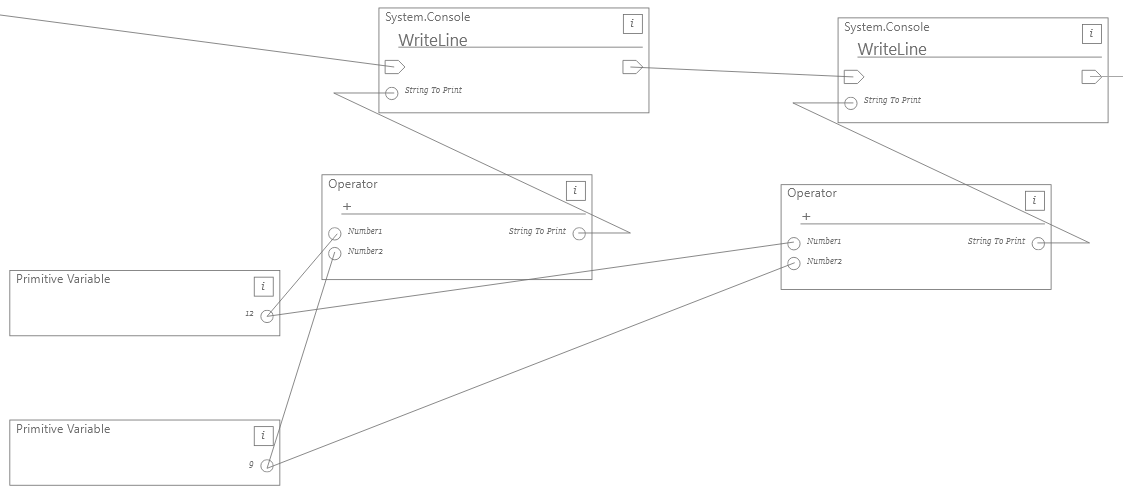
\includegraphics[width=1\textwidth]{exampl1.PNG}
    \caption{Example Visual Graph}
    \label{fig:exampl1}
\end{figure}

Those are:
\begin{itemize}
    \item \textbf{Fragile base class} \newline
          The problem comes from the ability to make changes to base class, which require all inheriting classes to be inspected for resulting faulty behaviours.
          For example here is example code for parent and child class in listing \ref*{fragile1}.
          \begin{lstlisting}[frame=single, label=fragile1, caption=Fragile Parent Class]
public class Parent{
    public virtual void DisplayToConsole(string message)
    {
        Console.WriteLine(message);
    }
    public virtual void LogToFile(string message){
        // TODO: write to file
    }
}
public class Child : Parent{
    public override void DisplayToConsole(string message)
    {
        LogToFile(message);
    }
}
    \end{lstlisting}
          The example program above is pretty straight forward - the Child class wants to log all requests to file instead. However, there is a problem of a fragile class in this program. Once Parent class was requested to also display message to console, so just 1 line modification was performed in the Parent class, which now completely halts the program, by locking it in the infite loop, see listing \ref*{fragile2}.
          \begin{lstlisting}[frame=single, label=fragile2, caption=Fragile Parent Class Backfired]
public class Parent{
    public virtual void DisplayToConsole(string message)
    {
        Console.WriteLine(message);
    }
    public virtual void LogToFile(string message){
        DisplayToConsole(message);
        // TODO: write to file
    }
}
public class Child : Parent{
    public override void DisplayToConsole(string message)
    {
        LogToFile(message);
    }
}
    \end{lstlisting}
          This seemingly harmless and thoughtful change to Parent class, suddenly breaks all existing programs that derive from this class if the decide to override the behaviour of DisplayToConsole with LogToFile.

    \item \textbf{The diamond problem} \newline
          The data model of OOP is based on inheritance. There is an example with fruits and decay. Naturally, all fruits slowly decay, they might have different rate and the rate might be affected by the environment. Although this might sound reasonable, there is another example with aluminum and decay. Aluminum is a metal, which will also decay over time. Just like the fruits, it has a different rate and slightly different conditions before it begins to decay. Furthermore, the decay operation, or 'function', is slightly different to that of a fruit. Despite that, both aluminum and fruit decay over time.
          The diamond problem, however, takes this matter a step further and asks a fundamental question 'is this inheritance even legal?'
          The following example in listing \ref*{diamond1} will address legality of inheritance.
          \newpage
          \begin{lstlisting}[frame=single, label=diamond1, caption=Inheritance Problem]
public class Student{
    public int StudyYear;
    public bool CanOpenDoor(int roomId){
        switch (roomId){
            case 1:
                return true;
            case 9:
                if (StudyYear > 2)
                    return true;
                return false;
            default:
                return false;
        }
    }
}

public class Professor{
    public bool CanOpenDoor(int roomId){
        switch (roomId){
            case 1:
            case 2:
            case 5:
            case 9:
                return true;
            default:
                return false;
        }
    }
}
    \end{lstlisting}
          In Student-Professor example, is it safe to say that a professor is a subclass of student? But if professor is child of a student class, the extra data such as 'StudyYear' would be obsolete and any methods that the class might have which are meant exclusively for students would somehow need to be locked.
    \item \textbf{Encapsulation} \newline
          Another problem with OOP is encapsulation. The following example in listing \ref*{encaps1} illustrates the issue.
          \begin{lstlisting}[frame=single, label=encaps1, caption=Encapsulation Problem]
public class Student{
    private List<int> OpenedDoors;
    public void OpenDoor(int doorId){
        // opens a door
        OpenedDoors.Add(doorId);
    }
    public List<int> GetOpenedDoors(){
        return OpenedDoors;
    }
}
    \end{lstlisting}
          When requesting a list of opened doors through method GetOpenedDoors, list of items is returned. Despite the variable being private, the returned list is, in fact, a reference to that list. This means that modifications to this returned list, which is a private variable in the class, will also affect class's variable OpenedDoors.
\end{itemize}

There are also C\# specific problems which we also go through:
\begin{itemize}
    \item \textbf{Little 'useful' accessibility modifiers} \newline
          In C\# there are multiple accessibility modifiers. All of modifiers, along with their access privileges, are displayed in figure \ref*{fig:accessc}.
          \begin{figure}[H]
              \centering
              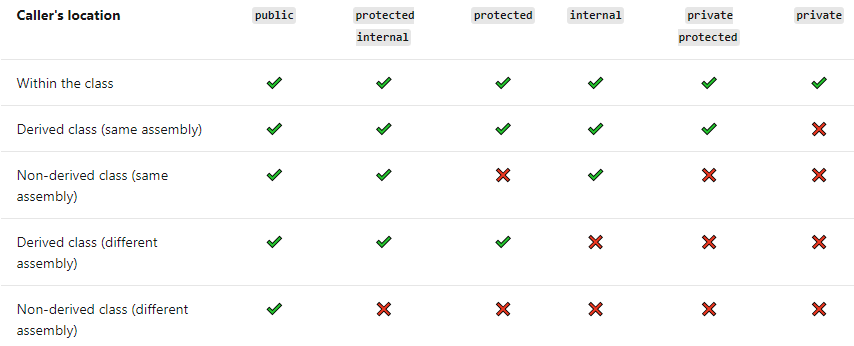
\includegraphics[width=1\textwidth]{access_csharp.PNG}
              \caption{C\# Access Modifiers}
              \label{fig:accessc}
          \end{figure}
          Unlike Java, C\# doesn't have a modifier to restrict access to a certain namespace, in fact, the only namespace-like restriction could be achieved through declaration of another assembly, in other words creating another C\# project and explicitly referencing this project. This is not at all useful, especially when projects are tied together and some access restrictions is absolutely necessary to keep codebase organized.
          Meanwhile Java addresses this problem by introducing package, which behaves like namespace. When the package is declared, it is enforced in the filesystem, meaning a file.java under folder some/folder must have a 'package some.folder' declaration in the source file, otherwise the entire java project will result in compilation error.
          Java offers fewer access modifiers but with greater impact due to existence of packages, those along with access levels can be seen in figure \ref*{fig:accessjav}.
          \begin{figure}[H]
              \centering
              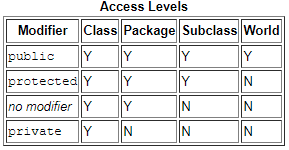
\includegraphics[width=1\textwidth]{access_java.PNG}
              \caption{JavaAccess Modifiers}
              \label{fig:accessjav}
          \end{figure}

    \item \textbf{Not enforced namespaces} \newline
          As previously stated, Java's namespaces, which are called packages, are enforced in the filesystem. When creating item.java file under com/apple folder, Java compiler will force 'package com.apple' declaration.
          C\#, however, doesn't enforce any namespaces onto the filesystem, which, consequently, creates a messy source code environment. Furthermore, unlike in Java, source code files in C\# are not enforced at all, meaning a single file can contain the codebase of the entire project, declaring namespaces one by one and classes within those namespaces, like in the example listing \ref*{enforce1}.
          \newpage
          \begin{lstlisting}[frame=single, label=enforce1, caption=Example File thisisok.cs]
namespace Root{
    public class Clazz{
        // some data

        // some methods
    }
}
namespace System.Numerics{
    public class Clazz{
        // some other data

        //some other methods
    }
}
            \end{lstlisting}
            Having ability to declare namespaces out of place, randomly and for any namespace hurts readability of the code. This makes a single namespace be composed by multiple files, quite literally, hidden across the project and may be even across assemblies.
    \item \textbf{Partial Classes} \newline
          Another problematic feature of the language is partial classes. When partial class is declared, this means it is can be completed somewhere else in a different file, possibly within a different folder. 
    \item \textbf{Multiple implementations of a Solution} \newline
          When there is a problem, there is an algorithmic solution. However, in case of C\#, the same solution can be implemented a thousand ways, but not because of the Turing-completeness of the language, but rather the design of the language. In the following listing \ref*{multi1}.
          \begin{lstlisting}[frame=single, label=multi1, caption=Example C\# File notok.cs]
public class Clazz{
    public int _Id;
    public int Id {get => _Id;}
    public int GetId(){
            return Id;
    }
    public int GetId1() => _Id;

}
          \end{lstlisting}
          In the above example, the problem is the following: 'Retrieve a field value \_Id'.
          The solution of the problem is a simple one - simply get the field value. However, an '\_Id' variable can be retrieved using 1 of 4 ways, using syntax of the language, in other words, the solution can be implemented in 4 ways. When the complexity of the problem grows and the complexity of the solution grows exponentially fast, the implementation should be limited to help programmer stay on course to the solution instead of creating extra overhead (in form of system design decisions) by providing extra implementation tools which impose extra decisions to be made by the programmer. Consider the example in listing \ref*{multi2}.
          \begin{lstlisting}[frame=single, label=multi2, caption=Simple get/set Example C\# File reallynotok.cs]
public class Clazz
{
    public int SomeVar { get => SomeVar - 1; private set { SomeVar = value; } }
    public void SetSomeVar(int value) =>
        SomeVar = ++value;
}
            \end{lstlisting}
          A simple getter/setter variable example is quite difficult to read and understand what the program is trying to achieve instantly. As the codebase grows and evolves, it becomes increasingly difficult to read the code.
\end{itemize}
In conclusion, features and design decisions in the list above, make C\# virtually impossible to navigate through without a proper IDE such as VSCode, Visual Studio, Eclipse, Rider or others.

This research has a few distinctive objectives it attempts to address:
\begin{itemize}
    \item A set of questions in the section \nameref{sec:motive}.
    \item Proposes a design for creating simple programs through G\# language.
    \item Presents implementation of G\# VPE.
\end{itemize}

// Aims of this research




\section{Background}
In this section, we will discuss how programming languages became what they are now, later, how they became abstract to accommodate extensibility.
Subsequently, we will discuss Object-Oriented Language C\# which is the language to which G\# will transpile.
It is important to understand why visual environments started to appear and what purpose did they serve. T
Finally, we will acknowledge and briefly discuss existing visual programming environments Blockly and 

\subsection{First abstract language}
The first ever abstract language appeared around 1969-1973 and it rapidly replaced assembly language which offered 'one-at-a-time' instruction in a semi-readable for human format. The C Programming Language quickly became a legend among programmers, especially those working on a very first UNIX operating system\cite{ritche_clang}.
The C programming language introduced a wide range of abstract paradigms that programmers could utilize to swiftly develop readable programs where they can orient freely and extend to their needs. Some of the examples of such paradigms include: struct, enum and array indexing with the following syntax:

\begin{lstlisting}[caption=C array indexing]
variable[2]
other_variable[0]
\end{lstlisting}

Programs that would otherwise require hours of revision and coding could be written in a matter of minutes, if not seconds. After C language, a major abstract language at a time, was standardized by ANSI, it became the primary language for most computing systems.

Despite being a standard for most, if not all, computing systems, the language was platform-specific, meaning different platforms would have specific implementations, hence compiled executables could only be run on the platforms for which executables were explicitly compiled. That way executables compiled for Windows would not run on MacOS/Linux Unix systems.

Unlike most, C language offers naked address referencing, meaning any given number could be converted into address in memory and backwards. This low level access to actual computer memory is strongly tied to memory leaks, critical security leaks, and even unwanted overflows that, if left unchecked, could violate kernel space from user space, which in turn could trigger kernel panic.\cite{6234805} Not only extremely low-level access that the C language provides poses severe vulnerability risk to the entire operating system, but it also requires significantly advanced memory management systems written by the applications' developers. In contrast, languages such as Java or C\# have built-in memory management that automatically frees memory when instances no longer accessible.
For these reasons C language simply did not offer enough abstraction, security, and flexibility to aid development of complex programs.\cite{schmidt_1977_some}

\subsection{Object-Oriented Programming}
Object-Oriented Programing, henceforth OOP, was primary focus of early stages of research because it is a paradigm that is used by a target language C\#. Expressing OOP data model, even in native, textual format proves to be troublesome. There are a few design flaws which heavily contribute towards rejecting OOP data model. 

For this research, a custom language has to be developed to accommodate all the needs of the visual language. This visual programming paradigm is the primary focus of this research. In the remaining subsections every design of the language will be discussed and explained in-depth. By the end of each subsection, there should be a clear understanding why those decisions came to be and also why the design was rejected.

\subsection{First Visual Programming Environments}
Visual Programming Environments (henceforth VPE) were introduced for educational purposes first appearing in 2003 for Intel's Computer Clubhouses where young could learn computer technologies. Original designs of scratch were solely intended for young by adding visual programmable elements that manipulate media on screen.\cite{demrkiran_2021_an}
Scratch UI uses sturdy design principles that achieve it's ultimate goal i.e. Single Window with multiple tabs ensures there is always visible primary components such as scene or code.

\subsection{Minecraft and Redstone}
Minecraft is a computer game that was introduced in 2009. Minecraft opened a new genre - Sandbox. Sandbox genre, effectively, allowed players to manipulate their environments and shape them visually how they see fit. Game introduced first few 'quests' that introduced player to the game, which then left player to explore world on their own. Minecraft is extremely successful, but not for a straightforward 'because of this and that' reasons. \cite{baek_2020_mining}
Why Minecraft game that has nothing to do with teaching and programming\cite{baek_2020_mining} (at the very least initially, it was designed for self-entertainment by creating stories using creative tools that the game provided\cite{booch_2013_from}) has a communities which focus heavily on implementing complex computing systems (even entire CPU architectures in Minecraft using nothing else but plain single-thread Redstone).\cite{matteson_2017_a}

\subsection{Transpilers, an upgrade to existing languages}
Transpilers take source code and compile into other source code. This is 'transpilation'.\cite{cifuentes_1998_assembly}

\subsection{Blockly and general-purpose VPE}
Blockly was a good take on general-purpose VPE. It uses transpiler principles to interpret visual representation of a code.\cite{7369000} It support wide range of target languages, however, currently, without specifically designed environment, Blockly, out-of-the-box, only supports few paradigms: functions, variables, arithmetic operations, flow control (loops, if statements) and a few more basic primitives like lists and color.\footnote{https://developers.google.com/blockly}
Blockly, natively, is only a set of theories and findings that build on top of preexisting VPE 'Scratch'.\cite{8120404} Despite it having rich and extensible documentation, Blockly is just a set of tools for creating VPEs.\cite{whitley_2006_evidence,bresson_2007_musical}





\section{Motivation}
\label{sec:motive}
How C achieved it's purpose?
Why has it became so popular?

How C represented basic programming constructs (for, while loops, if statements)?
When and why it fails?

Why Scratch became so popular?
How Scratch aims to achieve their aims?

Scratch is limited by Scratch VM.

Transpilers are interesting take on simplifying development.
Any attempts to generate code from Visual Programming Environments - refer to Blockly.

// merge into introduction

\section{System Design}
Previously mentioned transpilers were 'the next step' towards higher languages that might provide task-specific abstraction level and paradigms for easy development of said tasks.\cite{gribova_2013_ontology} For example, many game studios that started working in limited language such as Lua had to either rewrite their entire game on a different engine under different programming language. However, since introduction of transpilers that use higher-level or simpler languages to transpile to low-lever or complex languages, one of the most popular examples (in addition to mentioned Typescript-Javascript transpiler) being CSharp.lua\footnote{https://github.com/yanghuan/CSharp.lua} which takes c\# code and transpilers it into Lua code retaining most, if not all original language features such as reflection, polymorphism, encapsulation etc.

In this project, it was decided to utilize offline transpiler. This decision is motivated by strong presence of high-level heavily optimized languages such as Java, Javascript, C\#, Python, C++ and others. In contrast, the other choices were: Compiler and Interpreter.
Interpreter is an algorithm which uses calls and translates them one by one into bytecode, all of this 'interpretation' is happening at runtime and therefore creates huge overhead because every instruction the interpreter executes, essentially has to be looked up before it can be executed. Look up of interpreters is \textit{usually} capped at RAM latency, rather than CPU cache latency, meaning look up of instructions happens in RAM in worst case scenario.
Compiler both JIT and AOT require significant investment of time to design and implement from scratch. For purposes of this research, creating custom G\# to machine code compiler would be infeasible and would simply go outside of this project's scope.








\section{Language Design}
\label{sec:landes}
Currently there exist over 10 programming paradigms (in order of popularity): Object-Oriented Programming, Functional Programming, Imperative Programming, Procedural Programming, and others.
This research focuses on the Object-Oriented Programming because the target language is C\#, which is Object-Oriented. However, in the next section it will be discussed why such language design was

\subsection{Object-Oriented-Programming Design}


\subsection{Blockly and OOP}
A popular visual programming solution for real-world problems is Blockly, a visual programming environment based on Scratch. Example of Blockly is in figure \ref*{fig:blockly}.

\begin{figure}[H]
    \centering
    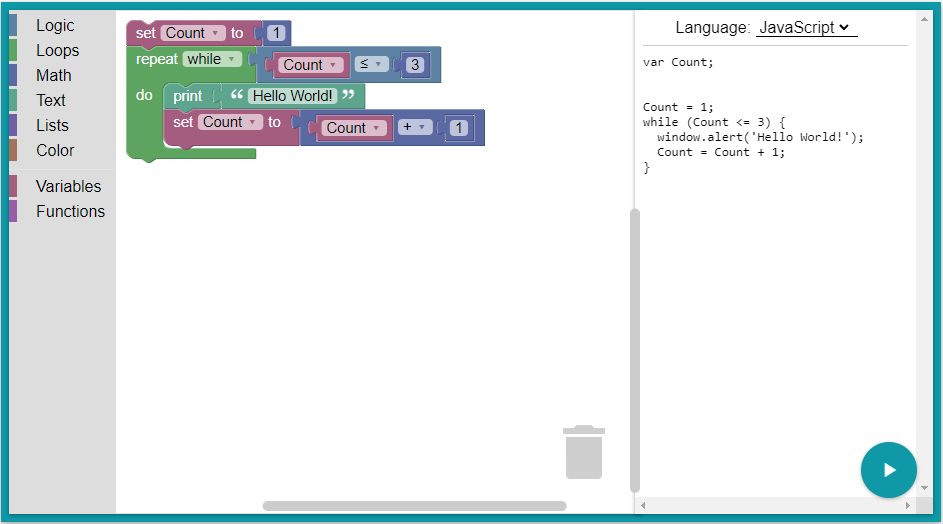
\includegraphics[width=1\textwidth]{blockly.PNG}
    \caption{Galaxy Editor}
    \label{fig:blockly}
\end{figure}


A few articles \cite{7369000, 8120404} pointed out some wrongs with Blockly, also, consequently, suggesting how some of the problems could be achieved. One of the problems is data, both variables and entire objects do not fit in block-based model that Blockly offers.

\cite{8120406}
\cite{1550357}


\subsection{StarCraft II inspired Behaviour Oriented Design}
Initially, the design was inspired by how StarCraft II's units behaviour builds up in the game. In the game StarCraft II, it is possible to create custom scenarios, called 'maps', using Galaxy Editor. The core gameplay of StarCraft II is also built using Galaxy Editor but with custom signing algorithm to make compiled scenario have 'Made by Blizzard' signature.
Galaxy Editor screenshot is in figure \ref*{fig:galaxy1}.
In the background is the primary editor, where the core elements of the map can be modified such as terrain, unit placements, regions for triggering events etc.
In front is the data editor, editor that the research is interested in. A close up of the editor and one of unit's behaviour lists is in figure \ref{fig:galaxy2}.

\begin{figure}[H]
    \centering
    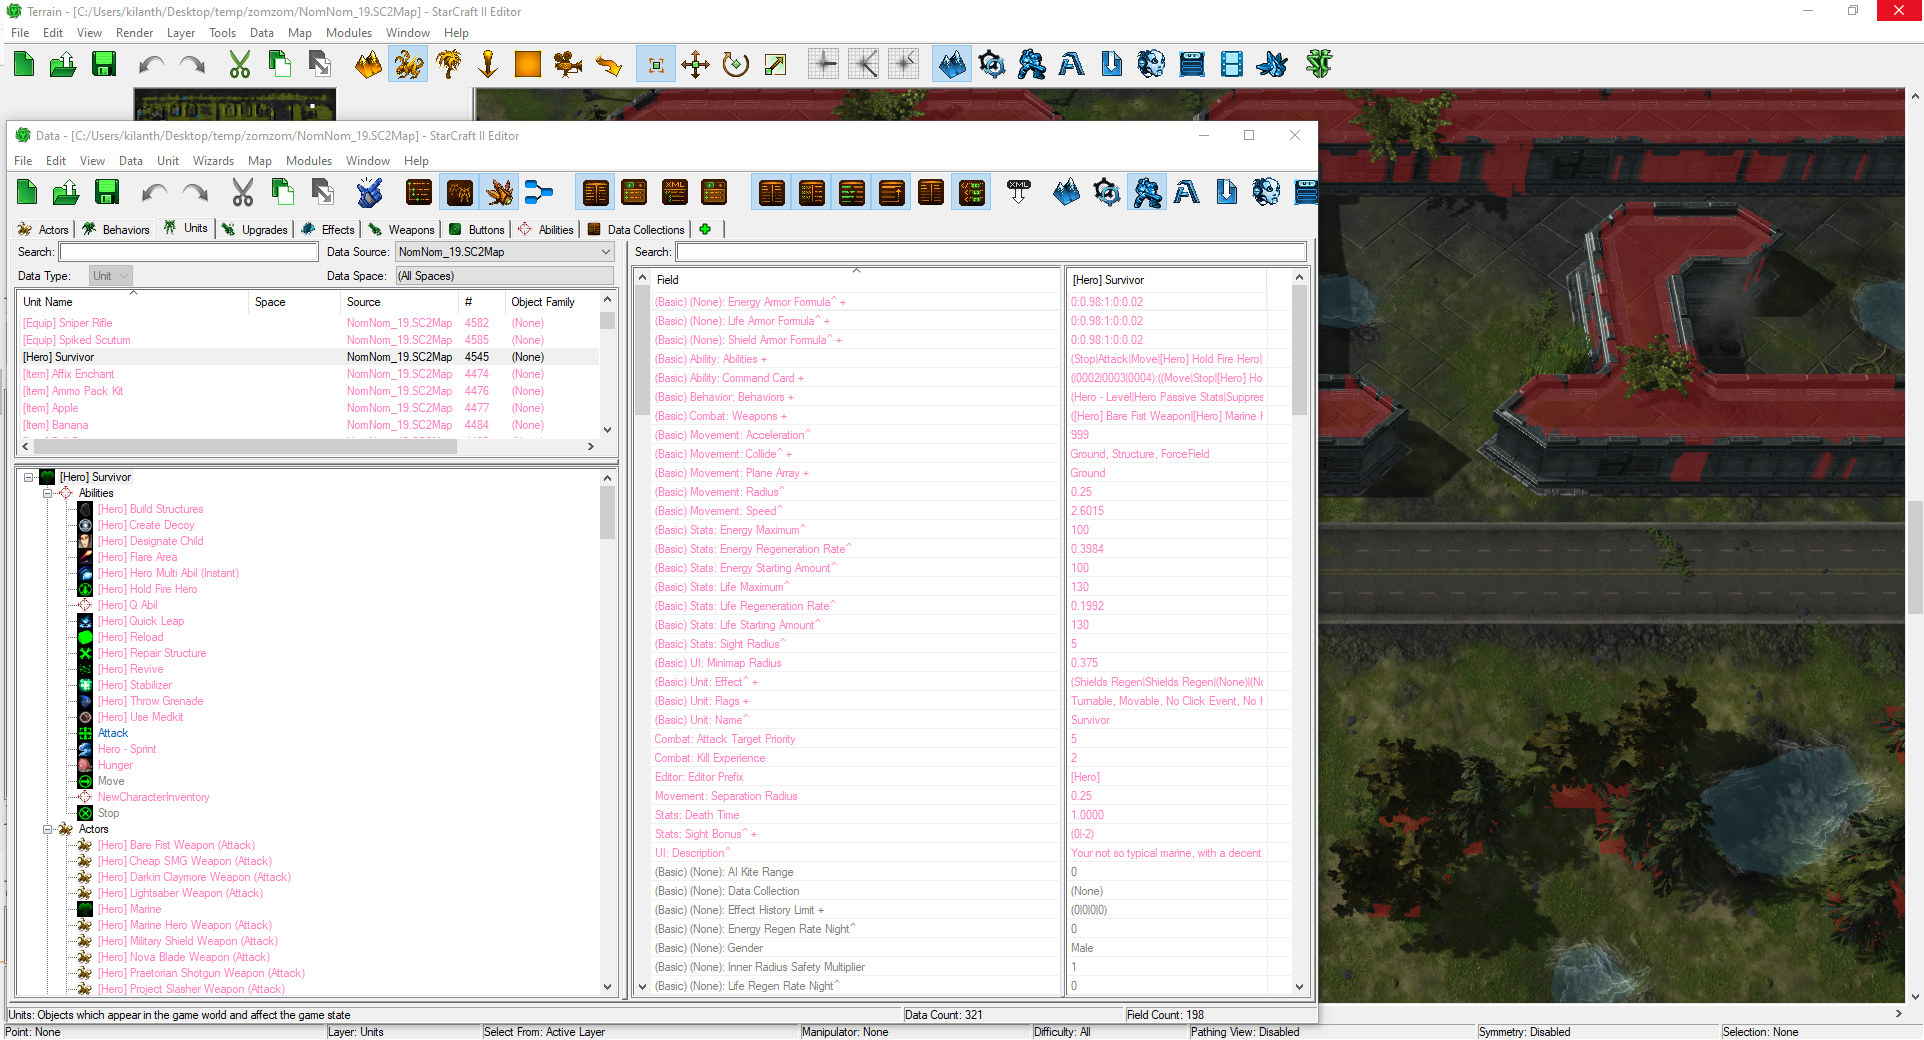
\includegraphics[width=1\textwidth]{galaxy_overview.PNG}
    \caption{Galaxy Editor}
    \label{fig:galaxy1}
\end{figure}

\begin{figure}[H]
    \centering
    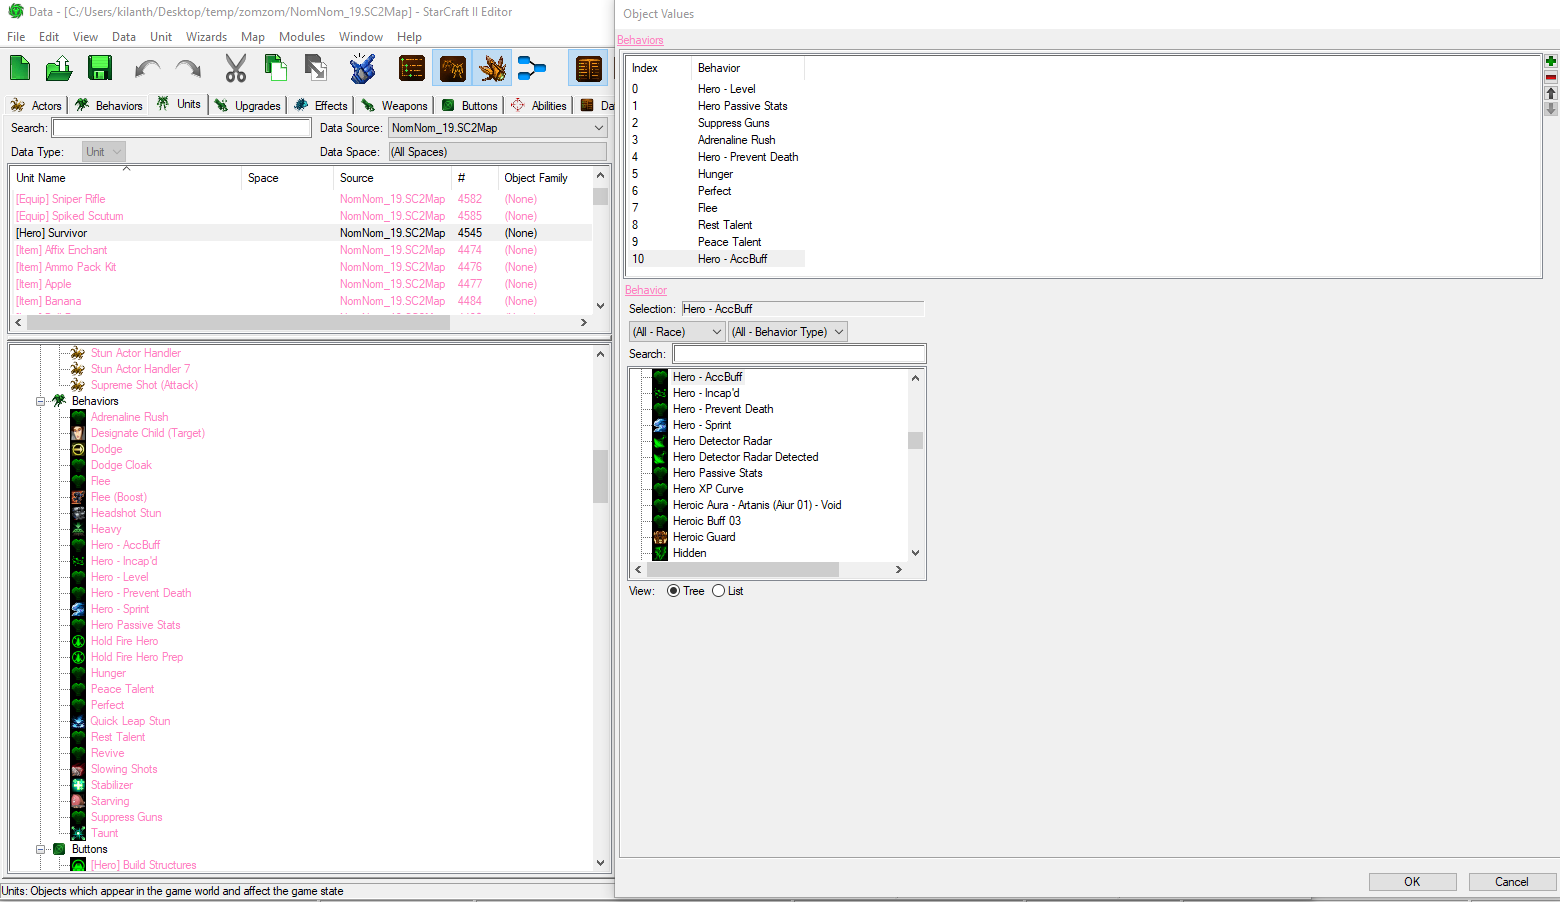
\includegraphics[width=1\textwidth]{galaxy_behaviours.PNG}
    \caption{Galaxy Data Editor}
    \label{fig:galaxy2}
\end{figure}

What is interesting is how any unit in the game - a player's primary character, enemy unit, or otherwise a neutral merchants that sells items have an array of behaviours that control unit's parameters, override their functionality or store custom data. For example, a unit might have a 'veterancy behaviour' enabling it to receive experience. Upon reaching a certain threshold, the unit will gain a new level, which might provide extra combat parameters or give an extra ability - all of it is highly configurable.
This kind of behaviour-enabling design is what allows objects to have multiple behaviours that would otherwise contradict OOP's data model. 

Research into Behaviour-Oriented-Design, henceforth BOD, \cite{d2857949266349429ebd6e5db6c1d3a3} has been already conducted and provided some results 'good potential', although, the prototype was 'less-advanced' due to time constrains.

\subsection{Node-like Shader Editor Design}
// write up\cite{kiper_1997_criteria, coronado_2020_visual}
\subsection{Unreal Engine Blueprints inspired Design}
// write up
\subsection{Stateless Node Editor}
// write up\cite{8120404}




\section{Implementation}
\subsection{Intermediate GryphonSharp Representation}
Intermediate G\# Representation (henceforth G\# IR) is a JSON-structured file containing code, data and metadata for both Transpiler and Node Editor.


\subsection{Incomplete Components}
Following subsections will include incomplete or unfinished components of this project. Generally, just like in the proposal of the GryphonSharp, the research was attempting to produce: Language Server (GryphonSharp-Overwatch), G\#-to-C\# Transpiler (GryphonSharp-Transpiler), and Visual Node Editor (GryphonSharp-vscode).
Every component is detailed and documented in the following subsections.

\subsubsection{Language Server}
Originally, Language Server, codenamed 'Overwatch', was planned to be implemented with VSCode language server protocol.\footnote{https://code.visualstudio.com/api/language-extensions/language-server-extension-guide}
The Overwatch language server handles multiple tasks listed below.
\begin{itemize}
    \item \textbf{Type-Safety Enforcer} \newline
          When user tries to connect nodes in the node editor, types of connectors are evaluated through Overwatch server request. Overwatch, being connected to Omnisharp server, will evaluate validity of type parsing and return boolean with TRUE value if parsing type is 'legal' for the connector, otherwise it will return FALSE, which will instruct node editor to highlight connection is 'illegal'. Highlight can either allow connection with red-error cross across illegal connection (can be seen in figure \ref{fig:badcon}) or prevent connection altogether and raise an error through message box (can be seen in figure \ref{fig:badconerror}).
          \begin{figure}[H]
              \centering
              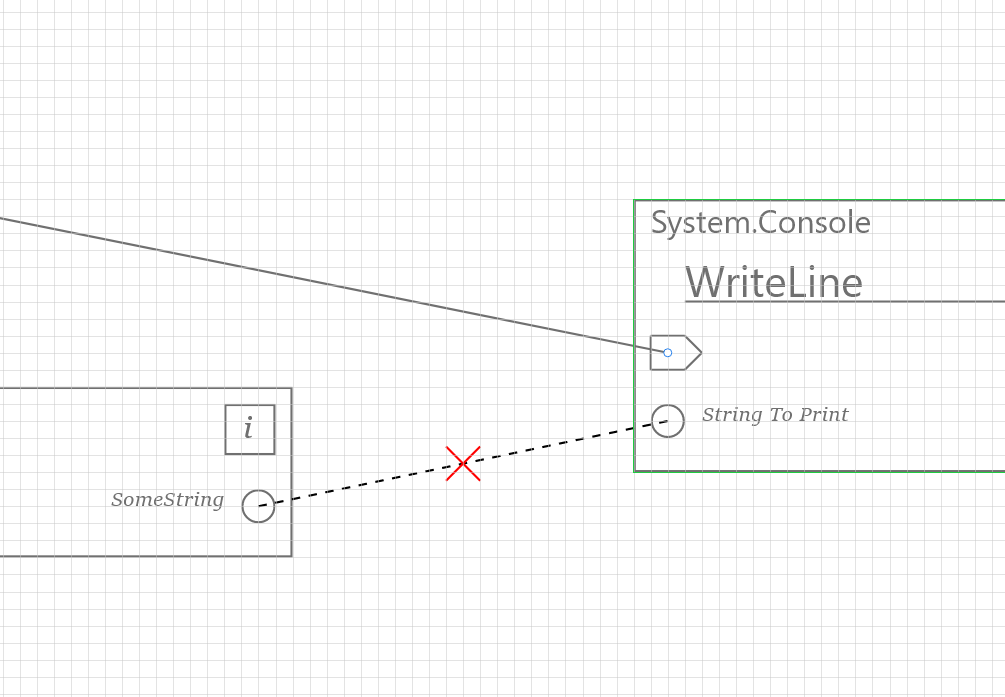
\includegraphics[width=1\textwidth]{illegalmove_cross.PNG}
              \caption{Illegal Connection}
              \label{fig:badcon}
          \end{figure}
          \begin{figure}[H]
              \centering
              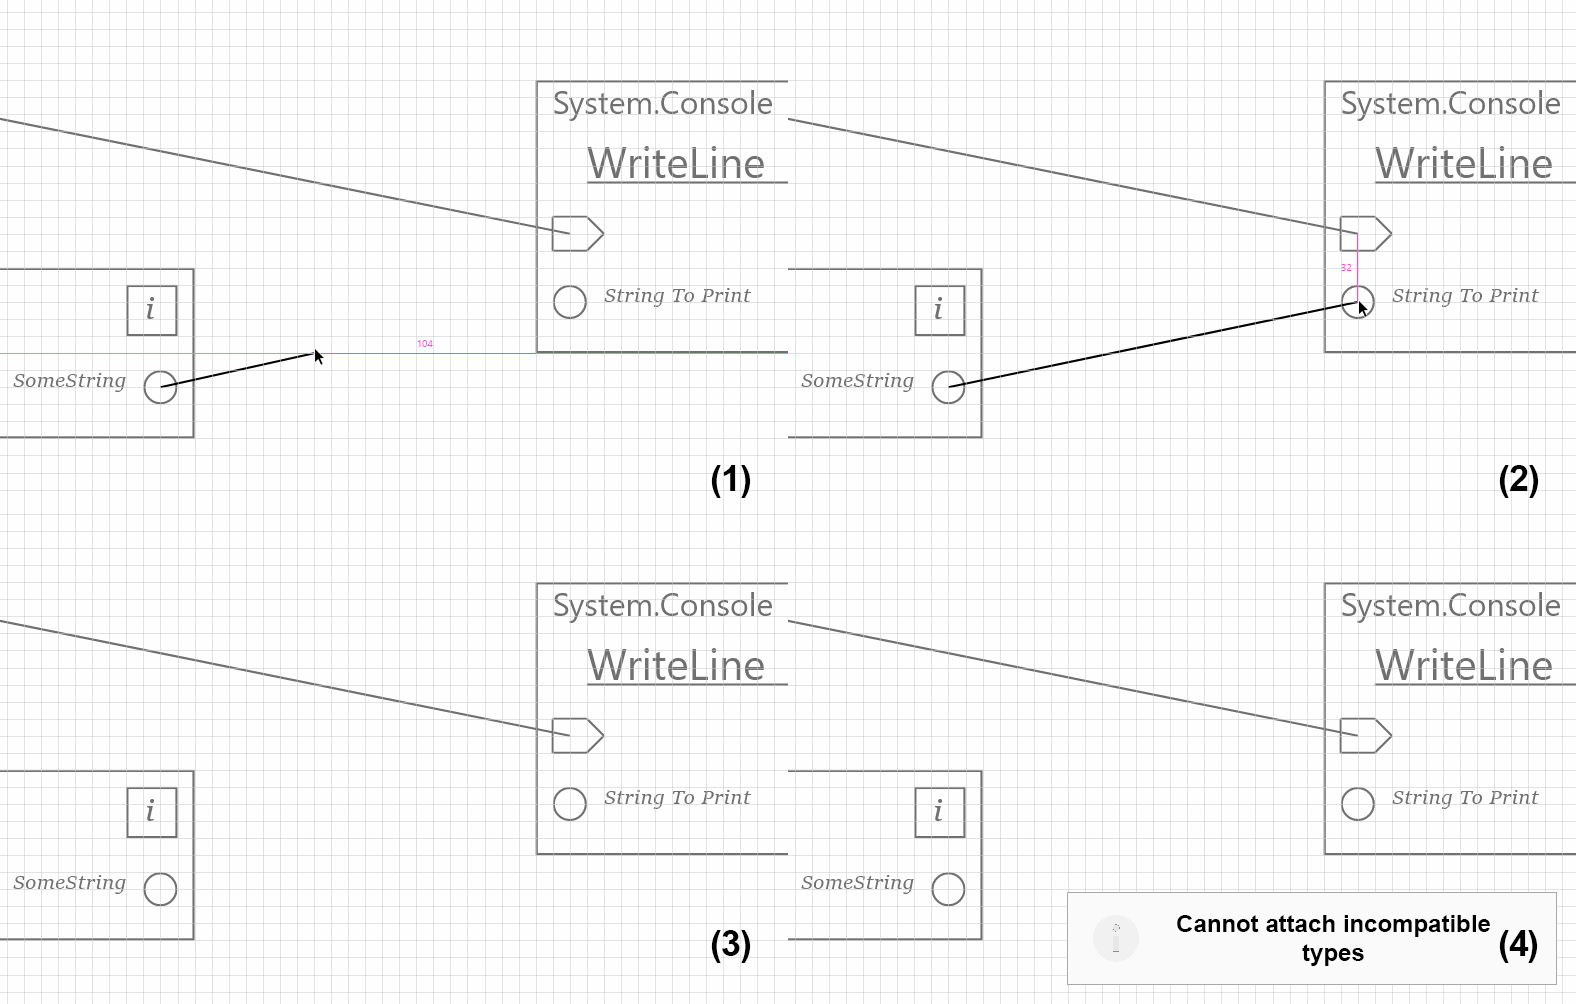
\includegraphics[width=1\textwidth]{illegalmove_message.png}
              \caption{Illegal Connection}
              \label{fig:badconerror}
          \end{figure}
    \item \textbf{Type Discovery} \newline
          When user attempts to parse a type into a empty space in the node editor, this will prompt user with function suggestions that match the parsed type.
    \item \textbf{Logic Evaluation} \newline
          When user constructs loops without exist clauses, such as while(true) loops or implement strange if statements, such as if(false), this will do a basic evaluation of the logic through existing tools in Omnisharp server.
    \item \textbf{Autocompletion} \newline
          When user types in a name of a function, variable, class or any other language construct, this will ask Omnisharp for Intellisense suggestions, which are then parsed into Node Editor for display.
    \item \textbf{Source Watcher} \newline
          When user makes changes to any of the files, Node Editor will notify VSCode of any workbench changes. These workbench changes are also parsed into language server. When the changes are made to source files or project files, language server will invoke G\#-to-C\# transpiler task.
\end{itemize}
\subsubsection{G\#-to-C\# Transpiler}
This is the actual transpiler that will convert G\# IR into C\# source code by the means of CodeDOM Microsoft package. CodeDOM allows construction of source code in readable format and supports all features of C\# language that are available to developers. CodeDOM is a powerful execution graph builder that supports C\# and IronPython transpilation. However, it can be defined, through a transformer factory, to translate into any other language according to the language's rules.
\subsubsection{Visual Node Editor}
Node Editor (in code is referred to as NE) is the primary focus of this research. Visual design of the editor is explained in-depth in section \nameref{sec:landes}. In this section, however, only the technical side of editor will be discussed.
Visual Node editor is an extension for a popular Electron app "Visual Studio Code"\footnote{https://code.visualstudio.com/}. Extension is written in typescript ES2015 and has 2 primary parts within the extension: Editor and Extension (sometimes referred to as simply frontend for Editor and backend for Extension).

Frontend of NE is an html page covered by a Konva canvas. Konvajs canvas is a high-performance canvas for drawing nodes. It has powerful API and has some very promising demos, some of which are: fully functional Google-like spreadsheets, react-konvajs which is used by some of high-end applications such as Polotno.\footnote{https://polotno.dev/}
User can manipulate nodes in the editor which will be written into a \lstinline[columns=fixed]{*.gs} file upon saving. G\# (or \lstinline[columns=fixed]{*.gs}) files contain JSON intermediate representation (IR) of G\#. This JSON contains a lot of metadata for both NE and transpiler. Furthermore, JSON is plaintext serializable data structure, meaning it can be used seamlessly with code transformation tools, version control tools, and even modified by hand.
Frontend of NE is written in Typescript, unlike extension it has slightly different compilation and deployment pipelines. Frontend has to be compiled 'for browser', since, as stated above, VSCode is only a chromium that displays webpage, but has a backend that allows it to interact with operating system. Unfortunately, TypeScript doesn't support compilation for Browser runtime, which means the code will have to be bundled. This projects takes advantage of Rollup bundler, which compiles Typescript code into ES6, but the transforms it through iteration of dependency tree. Source files, along with any referenced NodeJS libraries, bundled into a single \lstinline[columns=fixed]{*.js} file that can be instantly executed by NE frontend.
The second part of the NE is backend. Backend is written in Typescript as well and can be natively run by NodeJS runtime. Due to limitation and old technology used in VSCode, backend code is still compiled into deprecated CommonJS code. Extension code is then injected into a developer instance of VSCode. For release versions, code is bundled and executed as a module when added.

\section{Discussion}
This project was heavily time-constrained and therefore was left in a work-in-progress state.






\section{Appendix}

% \begin{figure}[H]
%     \centering
%     \includegraphics[width=1\textwidth]{}
%     \caption{Gantt Chart}
%     \label{fig:gantt}
%     \end{figure}

% \end{multicols*}
\pagebreak
\bibliographystyle{plain}
\bibliography{refs}
\end{document}
